\begin{figure}[ht]
\centering
\subfigure[]{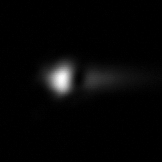
\includegraphics[width=4cm,keepaspectratio]{interference/figures/move/123-11.png}}
\subfigure[]{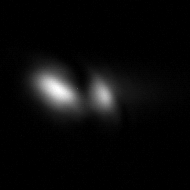
\includegraphics[width=4cm,keepaspectratio]{interference/figures/move/123-10.png}}
\subfigure[]{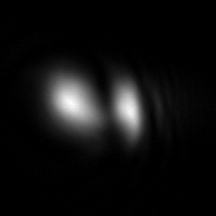
\includegraphics[width=4cm,keepaspectratio]{interference/figures/move/123-9.png}}\\
\subfigure[]{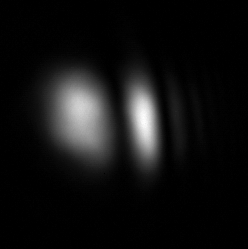
\includegraphics[width=4cm,keepaspectratio]{interference/figures/move/123-8.png}}
\subfigure[]{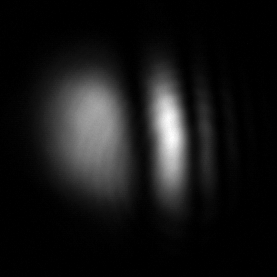
\includegraphics[width=4cm,keepaspectratio]{interference/figures/move/123-7.png}}
\subfigure[]{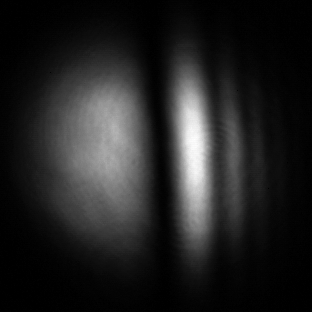
\includegraphics[width=4cm,keepaspectratio]{interference/figures/move/123-5.png}}\\
\subfigure[]{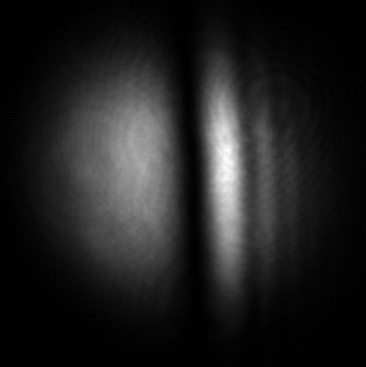
\includegraphics[width=4cm,keepaspectratio]{interference/figures/move/123-3.png}}
\subfigure[]{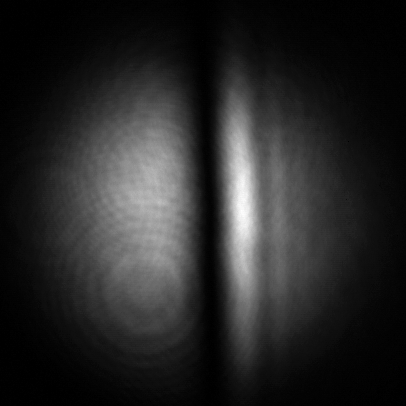
\includegraphics[width=4cm,keepaspectratio]{interference/figures/move/123-2.png}}
\subfigure[]{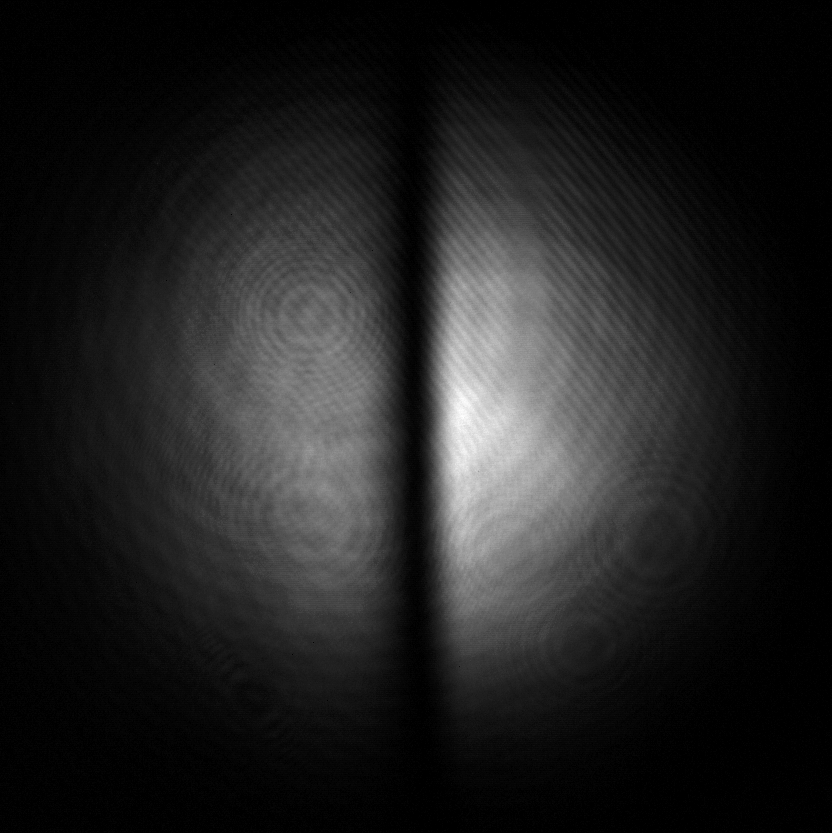
\includegraphics[width=4cm,keepaspectratio]{interference/figures/move/123-1.png}}
\caption{Images of the optical field in the specular direction as the focal
plane of $f_4$ is moved from (a), best focus, to (i), the far field.  All
images have been normalized relative to themselves.}
\label{fig:123up}
\end{figure}
